\documentclass[12pt]{article}

\usepackage{amsmath}    % need for subequations
\usepackage{graphicx}   % need for figures
\usepackage{verbatim}   % useful for program listings
\usepackage{color}      % use if color is used in text
\usepackage{subfigure}  % use for side-by-side figures
\usepackage{hyperref}   % use for hypertext links, including those to external documents and URLs
\usepackage{tikz}
\usepackage{pgfplots}

\begin{document}
\begin{figure}
\centering
% Created by tikzDevice version 0.7.0 on 2015-04-30 10:54:39
% !TEX encoding = UTF-8 Unicode
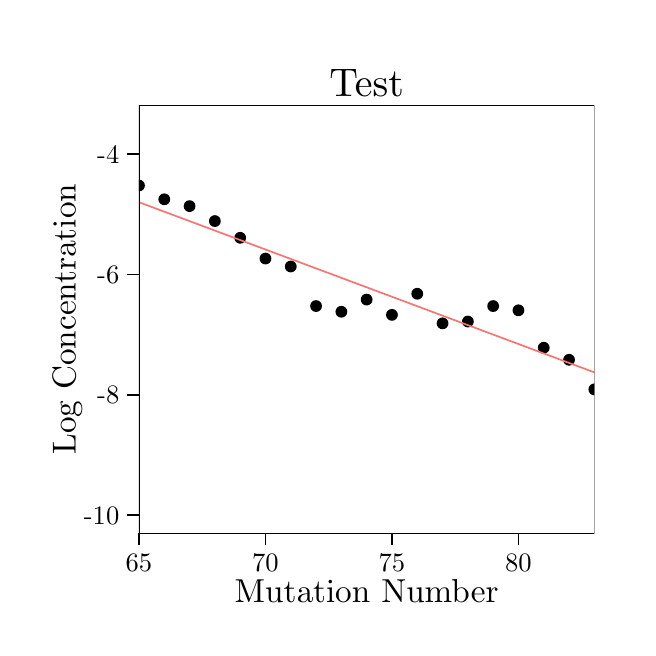
\begin{tikzpicture}[x=1pt,y=1pt]
\definecolor[named]{fillColor}{rgb}{1.00,1.00,1.00}
\path[use as bounding box,fill=fillColor,fill opacity=0.00] (0,0) rectangle (216.81,216.81);
\begin{scope}
\path[clip] (  0.00,  0.00) rectangle (216.81,216.81);
\definecolor[named]{drawColor}{rgb}{1.00,1.00,1.00}
\definecolor[named]{fillColor}{rgb}{1.00,1.00,1.00}

\path[draw=drawColor,line width= 0.6pt,line join=round,line cap=round,fill=fillColor] (  0.00,  0.00) rectangle (216.81,216.81);
\end{scope}
\begin{scope}
\path[clip] ( 40.22, 34.03) rectangle (204.76,188.82);
\definecolor[named]{fillColor}{rgb}{1.00,1.00,1.00}

\path[fill=fillColor] ( 40.22, 34.03) rectangle (204.76,188.82);
\definecolor[named]{fillColor}{rgb}{0.00,0.00,0.00}

\path[fill=fillColor] ( 40.22,159.77) circle (  2.13);

\path[fill=fillColor] ( 49.36,154.79) circle (  2.13);

\path[fill=fillColor] ( 58.50,152.32) circle (  2.13);

\path[fill=fillColor] ( 67.64,146.93) circle (  2.13);

\path[fill=fillColor] ( 76.79,140.88) circle (  2.13);

\path[fill=fillColor] ( 85.93,133.38) circle (  2.13);

\path[fill=fillColor] ( 95.07,130.51) circle (  2.13);

\path[fill=fillColor] (104.21,116.21) circle (  2.13);

\path[fill=fillColor] (113.35,114.15) circle (  2.13);

\path[fill=fillColor] (122.49,118.55) circle (  2.13);

\path[fill=fillColor] (131.63,113.03) circle (  2.13);

\path[fill=fillColor] (140.78,120.66) circle (  2.13);

\path[fill=fillColor] (149.92,109.97) circle (  2.13);

\path[fill=fillColor] (159.06,110.62) circle (  2.13);

\path[fill=fillColor] (168.20,116.21) circle (  2.13);

\path[fill=fillColor] (177.34,114.68) circle (  2.13);

\path[fill=fillColor] (186.48,101.16) circle (  2.13);

\path[fill=fillColor] (195.62, 96.80) circle (  2.13);

\path[fill=fillColor] (204.76, 86.11) circle (  2.13);
\definecolor[named]{drawColor}{rgb}{0.97,0.46,0.43}
\definecolor[named]{fillColor}{rgb}{0.97,0.46,0.43}

\path[draw=drawColor,line width= 0.6pt,line join=round,fill=fillColor] ( 40.22,153.73) -- (204.76, 92.25);
\definecolor[named]{drawColor}{rgb}{0.00,0.00,0.00}

\path[draw=drawColor,line width= 0.6pt,line join=round,line cap=round] ( 40.22, 34.03) rectangle (204.76,188.82);
\end{scope}
\begin{scope}
\path[clip] (  0.00,  0.00) rectangle (216.81,216.81);
\definecolor[named]{drawColor}{rgb}{0.00,0.00,0.00}

\node[text=drawColor,anchor=base east,inner sep=0pt, outer sep=0pt, scale=  0.96] at ( 33.11, 37.44) {-10};

\node[text=drawColor,anchor=base east,inner sep=0pt, outer sep=0pt, scale=  0.96] at ( 33.11, 80.87) {-8};

\node[text=drawColor,anchor=base east,inner sep=0pt, outer sep=0pt, scale=  0.96] at ( 33.11,124.31) {-6};

\node[text=drawColor,anchor=base east,inner sep=0pt, outer sep=0pt, scale=  0.96] at ( 33.11,167.74) {-4};
\end{scope}
\begin{scope}
\path[clip] (  0.00,  0.00) rectangle (216.81,216.81);
\definecolor[named]{drawColor}{rgb}{0.00,0.00,0.00}

\path[draw=drawColor,line width= 0.6pt,line join=round] ( 35.95, 40.74) --
	( 40.22, 40.74);

\path[draw=drawColor,line width= 0.6pt,line join=round] ( 35.95, 84.18) --
	( 40.22, 84.18);

\path[draw=drawColor,line width= 0.6pt,line join=round] ( 35.95,127.61) --
	( 40.22,127.61);

\path[draw=drawColor,line width= 0.6pt,line join=round] ( 35.95,171.04) --
	( 40.22,171.04);
\end{scope}
\begin{scope}
\path[clip] (  0.00,  0.00) rectangle (216.81,216.81);
\definecolor[named]{drawColor}{rgb}{0.00,0.00,0.00}

\path[draw=drawColor,line width= 0.6pt,line join=round] ( 40.22, 29.77) --
	( 40.22, 34.03);

\path[draw=drawColor,line width= 0.6pt,line join=round] ( 85.93, 29.77) --
	( 85.93, 34.03);

\path[draw=drawColor,line width= 0.6pt,line join=round] (131.63, 29.77) --
	(131.63, 34.03);

\path[draw=drawColor,line width= 0.6pt,line join=round] (177.34, 29.77) --
	(177.34, 34.03);
\end{scope}
\begin{scope}
\path[clip] (  0.00,  0.00) rectangle (216.81,216.81);
\definecolor[named]{drawColor}{rgb}{0.00,0.00,0.00}

\node[text=drawColor,anchor=base,inner sep=0pt, outer sep=0pt, scale=  0.96] at ( 40.22, 20.31) {65};

\node[text=drawColor,anchor=base,inner sep=0pt, outer sep=0pt, scale=  0.96] at ( 85.93, 20.31) {70};

\node[text=drawColor,anchor=base,inner sep=0pt, outer sep=0pt, scale=  0.96] at (131.63, 20.31) {75};

\node[text=drawColor,anchor=base,inner sep=0pt, outer sep=0pt, scale=  0.96] at (177.34, 20.31) {80};
\end{scope}
\begin{scope}
\path[clip] (  0.00,  0.00) rectangle (216.81,216.81);
\definecolor[named]{drawColor}{rgb}{0.00,0.00,0.00}

\node[text=drawColor,anchor=base,inner sep=0pt, outer sep=0pt, scale=  1.20] at (122.49,  9.03) {Mutation Number};
\end{scope}
\begin{scope}
\path[clip] (  0.00,  0.00) rectangle (216.81,216.81);
\definecolor[named]{drawColor}{rgb}{0.00,0.00,0.00}

\node[text=drawColor,rotate= 90.00,anchor=base,inner sep=0pt, outer sep=0pt, scale=  1.20] at ( 17.30,111.43) {Log Concentration};
\end{scope}
\begin{scope}
\path[clip] (  0.00,  0.00) rectangle (216.81,216.81);
\definecolor[named]{drawColor}{rgb}{0.00,0.00,0.00}

\node[text=drawColor,anchor=base,inner sep=0pt, outer sep=0pt, scale=  1.44] at (122.49,191.84) {Test};
\end{scope}
\end{tikzpicture}

\end{figure}
\begin{figure}
\centering
% Created by tikzDevice version 0.7.0 on 2015-04-30 08:26:53
% !TEX encoding = UTF-8 Unicode
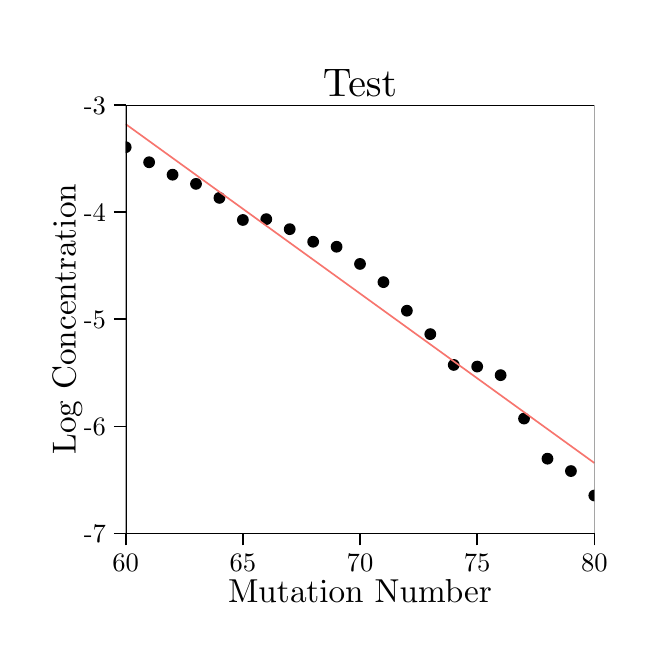
\begin{tikzpicture}[x=1pt,y=1pt]
\definecolor[named]{fillColor}{rgb}{1.00,1.00,1.00}
\path[use as bounding box,fill=fillColor,fill opacity=0.00] (0,0) rectangle (216.81,216.81);
\begin{scope}
\path[clip] (  0.00,  0.00) rectangle (216.81,216.81);
\definecolor[named]{drawColor}{rgb}{1.00,1.00,1.00}
\definecolor[named]{fillColor}{rgb}{1.00,1.00,1.00}

\path[draw=drawColor,line width= 0.6pt,line join=round,line cap=round,fill=fillColor] (  0.00,  0.00) rectangle (216.81,216.81);
\end{scope}
\begin{scope}
\path[clip] ( 35.42, 34.03) rectangle (204.76,188.82);
\definecolor[named]{fillColor}{rgb}{1.00,1.00,1.00}

\path[fill=fillColor] ( 35.42, 34.03) rectangle (204.76,188.82);
\definecolor[named]{fillColor}{rgb}{0.00,0.00,0.00}

\path[fill=fillColor] ( 35.42,173.61) circle (  2.13);

\path[fill=fillColor] ( 43.89,168.18) circle (  2.13);

\path[fill=fillColor] ( 52.36,163.68) circle (  2.13);

\path[fill=fillColor] ( 60.82,160.37) circle (  2.13);

\path[fill=fillColor] ( 69.29,155.30) circle (  2.13);

\path[fill=fillColor] ( 77.76,147.32) circle (  2.13);

\path[fill=fillColor] ( 86.22,147.62) circle (  2.13);

\path[fill=fillColor] ( 94.69,144.00) circle (  2.13);

\path[fill=fillColor] (103.16,139.45) circle (  2.13);

\path[fill=fillColor] (111.63,137.65) circle (  2.13);

\path[fill=fillColor] (120.09,131.44) circle (  2.13);

\path[fill=fillColor] (128.56,124.86) circle (  2.13);

\path[fill=fillColor] (137.03,114.53) circle (  2.13);

\path[fill=fillColor] (145.49,106.07) circle (  2.13);

\path[fill=fillColor] (153.96, 94.94) circle (  2.13);

\path[fill=fillColor] (162.43, 94.35) circle (  2.13);

\path[fill=fillColor] (170.90, 91.25) circle (  2.13);

\path[fill=fillColor] (179.36, 75.56) circle (  2.13);

\path[fill=fillColor] (187.83, 61.06) circle (  2.13);

\path[fill=fillColor] (196.30, 56.59) circle (  2.13);

\path[fill=fillColor] (204.76, 47.76) circle (  2.13);
\definecolor[named]{drawColor}{rgb}{0.97,0.46,0.43}
\definecolor[named]{fillColor}{rgb}{0.97,0.46,0.43}

\path[draw=drawColor,line width= 0.6pt,line join=round,fill=fillColor] ( 35.42,181.96) -- (204.76, 59.52);
\definecolor[named]{drawColor}{rgb}{0.00,0.00,0.00}

\path[draw=drawColor,line width= 0.6pt,line join=round,line cap=round] ( 35.42, 34.03) rectangle (204.76,188.82);
\end{scope}
\begin{scope}
\path[clip] (  0.00,  0.00) rectangle (216.81,216.81);
\definecolor[named]{drawColor}{rgb}{0.00,0.00,0.00}

\node[text=drawColor,anchor=base east,inner sep=0pt, outer sep=0pt, scale=  0.96] at ( 28.31, 30.73) {-7};

\node[text=drawColor,anchor=base east,inner sep=0pt, outer sep=0pt, scale=  0.96] at ( 28.31, 69.43) {-6};

\node[text=drawColor,anchor=base east,inner sep=0pt, outer sep=0pt, scale=  0.96] at ( 28.31,108.12) {-5};

\node[text=drawColor,anchor=base east,inner sep=0pt, outer sep=0pt, scale=  0.96] at ( 28.31,146.82) {-4};

\node[text=drawColor,anchor=base east,inner sep=0pt, outer sep=0pt, scale=  0.96] at ( 28.31,185.52) {-3};
\end{scope}
\begin{scope}
\path[clip] (  0.00,  0.00) rectangle (216.81,216.81);
\definecolor[named]{drawColor}{rgb}{0.00,0.00,0.00}

\path[draw=drawColor,line width= 0.6pt,line join=round] ( 31.15, 34.03) --
	( 35.42, 34.03);

\path[draw=drawColor,line width= 0.6pt,line join=round] ( 31.15, 72.73) --
	( 35.42, 72.73);

\path[draw=drawColor,line width= 0.6pt,line join=round] ( 31.15,111.43) --
	( 35.42,111.43);

\path[draw=drawColor,line width= 0.6pt,line join=round] ( 31.15,150.13) --
	( 35.42,150.13);

\path[draw=drawColor,line width= 0.6pt,line join=round] ( 31.15,188.82) --
	( 35.42,188.82);
\end{scope}
\begin{scope}
\path[clip] (  0.00,  0.00) rectangle (216.81,216.81);
\definecolor[named]{drawColor}{rgb}{0.00,0.00,0.00}

\path[draw=drawColor,line width= 0.6pt,line join=round] ( 35.42, 29.77) --
	( 35.42, 34.03);

\path[draw=drawColor,line width= 0.6pt,line join=round] ( 77.76, 29.77) --
	( 77.76, 34.03);

\path[draw=drawColor,line width= 0.6pt,line join=round] (120.09, 29.77) --
	(120.09, 34.03);

\path[draw=drawColor,line width= 0.6pt,line join=round] (162.43, 29.77) --
	(162.43, 34.03);

\path[draw=drawColor,line width= 0.6pt,line join=round] (204.76, 29.77) --
	(204.76, 34.03);
\end{scope}
\begin{scope}
\path[clip] (  0.00,  0.00) rectangle (216.81,216.81);
\definecolor[named]{drawColor}{rgb}{0.00,0.00,0.00}

\node[text=drawColor,anchor=base,inner sep=0pt, outer sep=0pt, scale=  0.96] at ( 35.42, 20.31) {60};

\node[text=drawColor,anchor=base,inner sep=0pt, outer sep=0pt, scale=  0.96] at ( 77.76, 20.31) {65};

\node[text=drawColor,anchor=base,inner sep=0pt, outer sep=0pt, scale=  0.96] at (120.09, 20.31) {70};

\node[text=drawColor,anchor=base,inner sep=0pt, outer sep=0pt, scale=  0.96] at (162.43, 20.31) {75};

\node[text=drawColor,anchor=base,inner sep=0pt, outer sep=0pt, scale=  0.96] at (204.76, 20.31) {80};
\end{scope}
\begin{scope}
\path[clip] (  0.00,  0.00) rectangle (216.81,216.81);
\definecolor[named]{drawColor}{rgb}{0.00,0.00,0.00}

\node[text=drawColor,anchor=base,inner sep=0pt, outer sep=0pt, scale=  1.20] at (120.09,  9.03) {Mutation Number};
\end{scope}
\begin{scope}
\path[clip] (  0.00,  0.00) rectangle (216.81,216.81);
\definecolor[named]{drawColor}{rgb}{0.00,0.00,0.00}

\node[text=drawColor,rotate= 90.00,anchor=base,inner sep=0pt, outer sep=0pt, scale=  1.20] at ( 17.30,111.43) {Log Concentration};
\end{scope}
\begin{scope}
\path[clip] (  0.00,  0.00) rectangle (216.81,216.81);
\definecolor[named]{drawColor}{rgb}{0.00,0.00,0.00}

\node[text=drawColor,anchor=base,inner sep=0pt, outer sep=0pt, scale=  1.44] at (120.09,191.84) {Test};
\end{scope}
\end{tikzpicture}

\end{figure}
\begin{figure}
\centering
\input{exp_simdata_flat.tex}
\end{figure}
\begin{figure}
\centering
\input{res_data_pos.tex}
\end{figure}
\begin{figure}
\centering
\input{res_data_neg.tex}
\end{figure}
\begin{figure}
\centering
\input{res_data_flat.tex}
\end{figure}
\end{document}